\documentclass[a4paper,12pt]{article}
\usepackage[toc,page]{appendix}
\usepackage{listings}
\usepackage{url}
\usepackage{graphicx}
\usepackage[skip=0pt]{caption}
\usepackage{multicol}
\usepackage{float}
\usepackage[margin=1in]{geometry}
%\usepackage{natbib}

\begin{document}

\renewcommand{\thelstlisting}{\thesection-\arabic{lstlisting}}
\renewcommand{\thefigure}{\arabic{section}-\arabic{figure}}
\setlength{\floatsep}{0pt plus 2pt minus 2pt}
%\setlength{\intextsep}{0pt plus 2pt minus 2pt}
%\setlength{\textfloatsep}{0pt plus 2pt minus 2pt}

\title{Introduction to Digital Libraries Assignment \#3}
\date{March 31, 2015}
\author{James Tate II}
\maketitle

\section{Introduction}
Assignment \#3 required comparing the downloaded webpages from assignment \#1 with and without the HTML
templates\cite{hw1}.
I attempted to remove HTML templates using jusText, a heuristic boilerplate removal tool\cite{justext}. The input
and output text of jusText was compared and jusText's performance was analysed.

\section{Methodology}
I wrote two scripts for this utility, both of which are available in my git repository on
GitHub\footnote{\url{https://github.com/jamesbtate/cs851-s15}}.

\subsection{jusText}
The first step of this assignment was to run the webpages through jusText. To facilitate this, I generated a couple
lists and wrote a utility. Listing 2.1 show how I generated a list of all files in my tweets directory.

\begin{lstlisting}[basicstyle=\ttfamily,caption={Generating list of files in tweets directory}]
    find ./tweets/ > tweets_file_list
\end{lstlisting}

Listing 2.2 shows how I generated the list of unique final URIs. The utility used is one I created in assignment
\#1.

\begin{lstlisting}[basicstyle=\ttfamily,caption={Generating list of unique final URIs}]
    ./summary.py -r tweets.summary.json -Mm 10000 \
        > uniq_final_uris
\end{lstlisting}

Both of these lists are hard-coded in the \emph{run\_boilerpipe.py} utility shown in Listing 2.3. This utility
identifies one representation of each unique final URI, and runs boilerpipe on that instance. It is necessary to
filter the input, because I carelessly downloaded multiple copies of the same resource in the first assignment.
The output from boilerpipe is saved in a \emph{boilerpipe.output} file in the same directory as the previously
saved representation.

\begin{lstlisting}[basicstyle=\ttfamily,caption={Running jusText}]
    ./run_boilerpipe.py
\end{lstlisting}

This utility makes one call to the jusText command in Listing 2.4 for each input file. The values
\emph{output-file} and \emph{input-file} were automatically replaced with the correct values on each call.

\begin{lstlisting}[basicstyle=\ttfamily,caption={Actual jusText command}]
    python -m justext -s English -o output-file input-file
\end{lstlisting}

\subsection{Word Counts}
The second part of this assignment asked for the frequency of terms in the input and output to jusText. To easily
calculate this data, I concatenated the unique downloaded representations into one file, and the same representations
after they were processed by jusText into another file. These concatenations are shown in Listing 2.5. The extra
\emph{echo ``''} is there to make sure any downloaded representations without a trailing newline are properly
delimited from the next representation. Otherwise, there would be a potential to erroneously combine the last word
of one document with the first word in the next document.

\begin{lstlisting}[basicstyle=\ttfamily,caption={Concatenating input and output data.}]
    grep "boilerpipe.output" tweets_file_list \
        | xargs cat > concat_boilerpipe
    while read line; \
        do cat "$line" >> concat_original; \
        echo "" >> concat_original; \
        done < uniq_uri_content_files
\end{lstlisting}

The two concatenations, \emph{concat\_boilerpipe} and \emph{concat\_original}, were processed twice each by the
\emph{word\_count.py} utility as shown in Listing 2.6. The default behaviour is to treat any term separated by
whitespace as a ``word'' and to count the frequency of each unique ``word,'' after converting all text to
lowercase. With the \emph{-l} flag, only consecutive letters, apostrophes and hyphens are treated as words.
Apostrophes and hyphens are only accepted if they immediately follow a letter.

\begin{lstlisting}[basicstyle=\ttfamily,caption={Concatenating input and output data.}]
    ./word_count.py concat_boilerpipe \
        > boilerpipe_words
    ./word_count.py -l concat_boilerpipe \
        > boilerpipe_words_letters-only
    ./word_count.py concat_original \
        > original_words
    ./word_count.py -l concat_original \
        > original_words_letters-only
\end{lstlisting}

\section{Statistics}

%\begin{figure}[H]
%    \centering
%    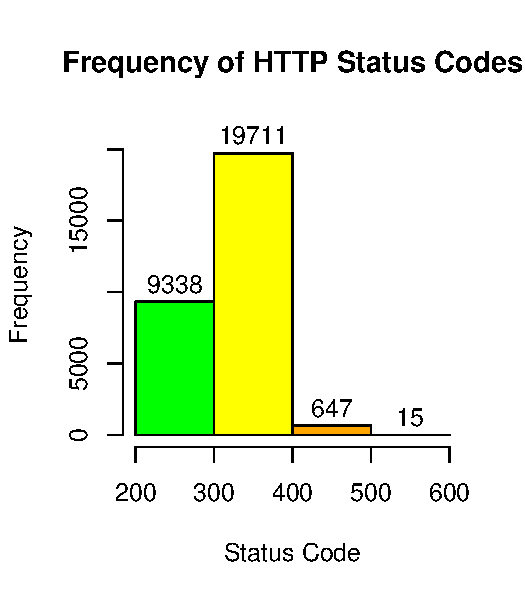
\includegraphics{stats/http_status_codes.pdf}
%    \caption{Frequency of HTTP status codes in histogram by sequential category.
%}
%\end{figure}

\clearpage
\begin{appendices}

\section{Streaming API Filter Keywords}
These keywords were selected arbitrarily. Keywords were added to the list until the streaming
API seemed to pull tweets at a strong, consistent rate.
\begin{multicols}{3}
\begin{itemize}
    \item python
    \item fsf
    \item foss
    \item coding
    \item programming
    \item fedora
    \item rhel
    \item dovetail
    \item woodworking
    \item blizzard
    \item snowstorm
    \item colorado
    \item virginia
    \item internet
    \item library
    \item libraries
    \item json
    \item lemonade
    \item woodchuck
    \item iasip
    \item league
    \item awesomenaut
    \item tf2
\end{itemize}
\end{multicols}

\end{appendices}




\bibliographystyle{plain}
\bibliography{../../cs751}

\end{document}
